\documentclass{article}
\usepackage{amsmath}
\usepackage[utf8]{inputenc}
\usepackage{graphicx}
\usepackage{dcolumn}
\usepackage{bm}
\usepackage{showkeys}
\usepackage{ragged2e}
\usepackage{cite}
\usepackage{authblk}
\usepackage{xcolor}
\usepackage{braket}
\newif{\ifmover}
\newif{\ifquitar}
\renewcommand{\Affilfont}{\small}
\newcommand{\notaL}[1]{{\color{orange}L: #1}}
\newcommand{\notaVA}[1]{{\color{orange}VA: #1}}
\newcommand{\notaVCG}[1]{{\bf \em \color{orange}VCG: #1}}
\definecolor{Addtext}{RGB}{0,0,255}
\begin{document}

%\title{Thickness optimization in wide range quasi omnidirectional multilayer
% structures}
\title{Optimization of wide-band quasi-omnidirectional 1-D photonic structures}
\author[1,2,3]{Victor Castillo-Gallardo\thanks{email: {\tt
			victor1\_1@hotmail.com}}}
\author[1,2,3]{Luis Eduardo Puente-D\'{i}az}
\author[4]{D. Ariza-Flores}
\author[3]{Hector P\'{e}rez-Aguilar}
\author[2]{W. Luis Moch\'{a}n\thanks{email: {\tt
			mochan@fis.unam.mx}}}
\author[1]{Vivechana Agarwal\thanks{email: {\tt
			vagarwal@uaem.mx}}}
\affil[1]{Centro de Investigaci\'{o}n en Ingenier\'{i}a y
Ciencias Aplicadas, Universidad del Estado de Morelos, Av.
Universidad 1001, Col. Chamilpa, Cuernavaca, Morelos 62209,
M\'{e}xico.}
\affil[2]{Instituto de Ciencias F\'{i}sicas, Universidad
Nacional Aut\'{o}noma de M\'{e}xico, Av. Universidad S/N,
Col. Chamilpa, 62210 Cuernavaca, Morelos, México.}
\affil[3]{Facultad de Ciencias Fìsico Matem\'{a}ticas,
Universidad Michoacana de San Nicol\'{a}s de Hidalgo, Av.
Francisco J. Múgica S/N 58030, Morelia, Mich., M\'{e}xico.}
\affil[4]{CONACyT-Universidad Aut\'{o}noma de San Luis
Potosì, Karakorum 1470, Lomas 4ta Secc, San Luis Potos\'{i},
S.L.P., 78210, M\'{e}xico.}
%\date{{\small {\today}}}
\maketitle


\begin{abstract}
Porous silicon (PS) is a very versatile material for developing optical
devices based on multilayered structures, since high and low porosity layers
can be synthesized by a simple electrochemical technique. We
maximize the reflectance $\braket{R}$ \notaL{El promedio no depende
  de lambda ni theta, y prom es castellano}   of PS-based
mirrors  averaged over a wide wavelength
and angular range, for different
porosity contrasts, and we minimize their thickness. Optimization is
performed in the visible (Vis) and near infrarred (NIR) regions of the
electromagnetic spectrum. We design the mirrors using \textit{chirped}-type
structures and by \textit{stacking} sub-mirrors. We found \notaL{No
  estoy seguro del tiempo} that
chirped structures were better suited for the Vis stacked
sub-mirrors for the NIR region. We design, fabricate and test some
optimized omnidirectional structures with less than 100
periods.
\end{abstract}

\section{Introduction}

Photonic crystal (PC)-based \notaL{Lo cambié de PhC, pues en otros
  casos abrevias photonic con sólo la P, como en PBG, no PhBG.}
structures have been extensively investigated due
to their light controlling properties \cite{Joannopoulos2008,Goyal2018}.
Photons entering a PC interact with its periodically varying dielectric constant and
are consequently organized into photonic bands. Analogous to electrons in a
crystal, their propagation will be forbidden if their energy lies
within certain regions known as photonic band gaps (PBG's). Thus, the
PC behaves as a mirror if illuminated by light with frequencies
withinin a PBG. For several applications it is useful to fabricate
{\em ommnidirectional} mirrors with a wide band gap.  The use of metallic
mirrors is limited due to their relatively large absorption at
visible and near infrared frequencies.  An attractive alternative
consists of low-absorption dielectric
structures,  which may be designed for specific frequency
ranges. One-dimensional (1D) and two-dimensional (2D) PCs have
applications in optoelectronics, optical telecommunications and computing,
laser technology \cite{Lopez2003,Masaya2010}, and radiative cooling applications
\cite{Kumar2020}. The simplest 1D-PC is composed of a finite number
of periodically alternating
layers of high $n_{H}$ and low $n_{L}$ refractive indices, with
corresponding thicknesses $d_H$ and $d_L$ chosen so that their optical
thicknesses of is quarter-wavelength
$n_{H}d_{H}=n_{L}d_{L}=\lambda_{0}/4$ at some chosen nominal
wavelength $\lambda_{0}$. This yields a {\em Bragg mirror} (BM)
which might have a large PBG including an omnidirectional gap if the contrast $n_H/n_L$
and the number of periods are large enough. Mirrors with high
reflectance within a wider frequency range may be engineered by
using different nominal wavelengths for different layers.
One way to obtain such structures is to gradually change the width of
the layers as a function of their depth, producing
\textit{chirped}-type \cite{Zipock1997}
structures. An alternative is to stack BM's, such that their PBG
overlap each other, resulting in a wider high-reflection band
\cite{Xifre2009}.
\notaL{No me convence la redacción. ¿No la revisó Vivechna?} \notaL{Para un
  espejo de Bragg, el ancho de banda de reflexión coincide (a incidencia normal)
  con la brecha prohibida, pero para los 'chirped' y los 'stacked',
  que no son periódicos, tal vez 'brecha prohibida' no es un buen
  término. Más bien, queremos hablar del ancho de banda del espejo,
  i.e., la región en que es buen reflector.}

Till now, different deposition techniques have been used to obtain omnidirectional
BM (ODBM) that operate on the visible and near infrared (Vis-NIR) range of the
electromagnetic spectrum. For example, Chen et al. \cite{Chen1999},
\notaL{Hay que checar que la puntuación vaya después de las citas,
  para este estilo de citas entre corchetes} have
reported an ODBM of about 70 nm in the NIR range with 6-pairs  of
TiO$_{2}$/SiO$_{2}$ layers deposited with a sol-gel method. Park et al., \cite{Park2003}
used molecular beam epitaxy to grow a stack of four pairs of GaAs/AlAs layers,
followed by its conversion to
GaAs/Al$_{2}$O$_{3}$ layers by selective
oxidation of the AlAs layers, to obtain an ODBM with a band from 710 to 950
nm. On the other hand, DeCorby et al. \cite{DeCorby2005}, fabricated mirrors by
coupling multiple layers of Ge$_{33}$As$_{12}$Se$_{55}$ chalcogenide glass and
polyamide-imide polymer, deposited by thermal evaporation and spin-casting
respectively, to obtain a 150 nm wide omnidirectional band centered at
1750 nm. Furthermore, Jena et al., \cite{Jena2019}
used sequential asymmetric bipolar pulsed DC magnetron sputtering (for TiO$%
_{2}$ layers) and radio frequency magnetron sputtering (for SiO$_{2}$
layers) to generate TiO$_{2}$/SiO$_{2}$ 1D-PC's and achieved ODBM from
592 to 668 nm. However, these techniques are expensive and they
require sophisticated equipment and long fabrication times. Using PS
is an attractive alternative, as PS may be fabricated by simple
electrochemical etching during short times of
crystalline Si in a hydrofluoric acid based electrolyte, to obtain the
sponge-like nanostructure composed of Si and air. By modulating in
time the applied current, the porosity of the PS, and thus its
refractive index, can be modulated
along its depth. This allows the design and fabrication of 1D-PC's with PS, to
control the propagation of light in a dielectric medium. The low cost and
ease of fabrication of PS make it an excellent candidate to develop
multilayered optical devices \cite{Xifre2015,Pavesi2000}.
Although optical filters \cite{Estevez2009,Ariza2014} are the most common
application of PS PC's, they have also been widely used as chemical
sensors \cite{Giusseppe2011,Agarwal2018}, waveguides \cite{Hussel1997} and
for photoluminescence control \cite{Antunez2014}. Recently, the study of
quasi-omnidirectional Bragg mirrors has
increased due to their possible application
as a flat lens \cite{Kozar2017,Cheng2018}.\notaL{Lens o mirror, no
  puede ser ambas? De verdad esto es lo que más lo ha popularizado?}
PS based dielectric
optical filters, quasi-ODBM and ODBM have been extensively studied in different
regions of the electromagnetic spectrum, such as the ultraviolet (UV)
\cite{Jimenez2020}, visible \cite{Ariza2012}, and (NIR)
\cite{Bruyant2003}. However, to obtain the desirable high index of refraction
contrast, layers of high porosity have to be employed, so that the
resulting structures may be fragile, making large structures, with a
very large number of layers, unfeasible. For this reason, in this work
we study different strategies to produce photonic mirrors
that have a large reflectance over a wide band-width with a relatively
small thickness and refractive index contrast. Specifically, our aim
is to maximize the reflectance $R$ averaged over a wide range of
wavelengths $\lambda$ and angles of incidence $\theta$.

This paper is organized as follows. In Sec. \ref{s:theory} \notaL{No uses números,
  usa referencias a etiquetas para numerar y referir todo} we develop the
methods used to design and calculate the reflectance spectra of the PS
multilayered structures such as chirped structures and mirror
stacks. In Sec. \ref{s:exp} we provide details about the
fabrication of these structures. In Sec. \ref{s:res} we present the numerical
and experimental results for our proposed structures and compare
them to previous reports. We obtained significantly larger band-widths
with significantly thinner structures. \notaL{Dejo para resultados y
  conclusiones los detalles de con quién comparamos y qué salió.}
Finally, we discuss our conclusions in Section \ref{s:conc}.

\section{Theory}\label{s:theory}

\notaL{Pon etiquetas a todo para poderlo referir}
For the analysis of the propagation of electromagnetic fields through
multilayer systems it is usual to employ the transfer matrix
method\notaL{reference}. Assuming the system is 1D, with variations
only along the $z$ directions, and that the polarization of light is either
transverse electric (TE) or transverse magnetic (TM)\notaL{si no, la matriz
  sería de 4x4}, the
transfer matrix $M\left(z_{2},z_{1}\right)$ is
a 2x2 matrix that relates the components of the electric $E_{\| }$
and magnetic  $H_{\|}$ fields parallel to the $xy$ plane
evaluated at $z_2$ to their value at $z_{1}$,
\begin{equation*}
\left(
\begin{array}{c}
E_{\|} \\
H_{\| }%
\end{array}%
\right) _{z_{2}}=M\left( z_{2},z_{1}\right) \left(
\begin{array}{c}
E_{\| } \\
H_{\| }%
\end{array}%
\right) _{z_{1}}.
\end{equation*}%
Many equivalent formulations have been proposed to obtain and use $M$
\cite{Mochan1987,Ortiz2020,Chavez2020}. Here we use a recently developed formalism
for the numerically stable calculation of the reflectance of large
multilayer systems, as
proposed by Puente-Díaaz, et al. \cite{Puente2020}, summarized in the
supplementary information. The
explicit expressions for the optical coefficients are:
\begin{equation}
r=\mp \frac{Z_{0}M_{11}+M_{12}-Z_{0}Z_{s}M_{21}-Z_s
M_{22}}{Z_{0}M_{11}-M_{12}-Z_{0}Z_{s}M_{21}+Z_{s}M_{22}},  \label{rBloch}
\end{equation}%
and
\begin{equation}
t=\frac{2Z_{\alpha
  }}{Z_{0}M_{11}-M_{12}-Z_{0}Z_{s}M_{21}+Z_{s}M_{22}},  \label{tBloch}
\end{equation}%
where $M_{ij}$ \notaL{Quité las tildes, pues hubiera sido necesario
  explicarlas, y no creo que sean importantes para el lector} are the elements
of the transfer matrix which transfer
the fields from its surface interface with vacuum at $z_0$ towards the
substrate at $z_s$,  $Z_0$ is the surface impedance of vacuum and $Z_s$ is the
surface impedance of the substrate, and we define $r=F_r/F_i$ and $t=F_t/F_i$ in terms
of the reflected and transmitted fields, where we choose the $F$'s as electric
fields for (TE) polarization and magnetic fields
for transverse magnetic polarization (TM). The upper sign $-$ in
Eq. (\ref{rBloch}) and the subscript $\alpha =s$
in Eq. (\ref{tBloch}) are chosen for the case of TE polarization, while
the lower sign $+$ and the subscript $\alpha =0$ correspond to TM
polarization, respectively.
The reflectance is given by
$R=|r|^{2}$ and the
transmittance by $T=\beta \left\vert t\right\vert ^{2}$ with $\beta
=\text{Re}Z_{0}/\text{Re}Z_{s}$ for TE polarization and $\beta =\text{Re}Z_{s}/\text{Re}Z_{0}$ for
TM polarization.\notaL{En el cálculo, ¿tomaste las partes reales? No
  estaban en la fórmula} The complex refractive index of the porous
layers were obtained through the Bruggeman's effective medium theory, which
has been reported to adequately reproduce the PS optical parameters
\cite{Giusseppe2011,Pap2006,Estrada2018}.

\notaL{Creo que esto debería estar más adelante:
  After the next section, two techniques are developed to design multilayer
photonic structures. In the first, the wavelength ($\lambda _{j}$), at which
the $j$-th period of the structure is designed, is modulated by an
increasing function. This can be as simple or complex as you like. The
proposed function was optimized with the Minuit module of PDL (Perl Data
Language) \cite{minuit}. The other technique for proposing highly reflective
structures over a wide region of the electromagnetic spectrum is to stack
sub-mirrors tuned to different wavelengths. For each sub-mirror the
dispersion relation is analyzed.
}

\section{Experimental details}\label{s:exp}

Some of the proposed photonic structures were synthesized through anodic
etching of a (100) oriented, $p$-type Boron doped, crystalline Si wafer with
resistivity 0.002-0.005 $\Omega \cdot $cm, under galvanostatic conditions
\cite{Canham1990,Escorcia2007}. The electrochemical anodization process was
performed at room temperature, with an electrolyte of aqueous
hydrofluoric acid (HF) (48$\%$ of
wt) and ethanol (99.9$\%$ of wt) in 1:1 volumetric proportion, respectively.
With this electrolyte, the minimum and maximum porosities that can be
obtained are 35$\%$ and 76$\%$ \notaL{Creo que se puede quitar de
  aquí, pues lo discutes abajo:(gravimetrically obtained)}, using
current densities of 0.5 and $305\text{mA}/\text{cm}^{2}$,
respectively. However, as it is not desirable to use very high
porosity contrasts due to structure fragility and electrolyte
diffusivity problems \cite{Ariza2011}, the current
densities were chosen as 35 and $305\text{mA}/\text{cm}^{2}$, with
corresponding
porosities of 51\% and 76\%, respectively. The porosity was calibrated
\notaL{Creo que no muestras curvas de calibración: calibration curves were
acquired} through a gravimetric technique as follows: single layers of porous
silicon were synthesized under similar conditions applying a constant
current for a time \notaL{cuánto tiempo para la calibración?}  and were weighed to
obtain their mass $m_i$
before ($m_{1}$) and after ($m_{2}$) the electrochemical attack, and after
dissolving the already formed porous silicon layer ($m_{3}$), to obtain
the porosity as $p=(m_{1}-m_{2})/(m_{1}-m_{3})$ \cite{Pap2006}.
The etching
rate of PS was obtained by synthetizing single layers under similar
conditions and measuring their thicknesses through Scanning Electron
Microscopy (SEM). Absolute reflectivity measurements were carried out
with a Perkin Elmer Lambda 950 UV/Visible spectrophotometer with a variable
angle universal reflectance accessory (URA) for different incident
angles $\theta _{i}=10^{\circ }$, $20^{\circ }$, $30^{\circ }$,
$40^{\circ }$, $50^{\circ }$ and $60^{\circ }$ using non-polarized light. The maximum and
minimum values of $\theta _{i}$ were constrained by the angular range of the
equipment accessory URA.

\section{Results and discussion}\label{s:res}

In this section we presents optimized calculations of the reflectance
of different multilayered omnidirectional wide-band mirrors and we
compare the results to spectra taken from
the corresponding samples at several angles of
incidence. Sec. \ref{ss:chirped} is devoted to chirped-type Bragg
mirrors while Sec. \ref{ss:stacked} is devoted to structures made of
stacked sub-mirrors.

\notaL{Quizás esto se pueda incluir por aquí.:
  After the next section, two techniques are developed to design multilayer
photonic structures. In the first, the wavelength ($\lambda _{j}$), at which
the $j$-th period of the structure is designed, is modulated by an
increasing function. This can be as simple or complex as you
like. {\tiny The
proposed function was optimized with the Minuit module of PDL (Perl Data
Language) \cite{minuit}.} The other technique for proposing highly reflective
structures over a wide region of the electromagnetic spectrum is to stack
sub-mirrors tuned to different wavelengths. For each sub-mirror the
dispersion relation is analyzed.
}
\subsection{Chirped-type Bragg mirrors}\label{ss:chirped}

Here we study multilayered structures where the thicknesses for each
pair $j=0\ldots N_p$ of layers are tuned to a wavelength $\lambda_j$ which changes
gradually with the depth of the layer, according to
\begin{equation}
\lambda_{j}=\lambda_{\min }+\left(\lambda_{\max }-\lambda_{\min}\right) f(j/N_p)),\label{Dis}
\end{equation}%
where $\lambda_{\min }$ and $\lambda_{\max }$ are the minimum and {\em
  design} wavelengths respectively, $N_p$ is the index of the deepst
pair of layers and $f(x)$ is some smooth function
that goes from 0 to 1 as its argument goes from surface ($x=0$) to the
substrate ($x=1)$. We only consider increasing functions $f$ due to
the high absorption of PS in the ultraviolet region
which decreases in the visible and becomes negligible in the near
infrared, so, the
first periods are syntonized in the UV-Vis regions. We consider the
following classes of functions:
\begin{equation}
f_{1}\left( x\right) =x^{\alpha },  \label{F1}
\end{equation}
\begin{equation}
f_{2}\left( x\right) =A\left( x^{\alpha }+x^{\beta}\right)
\label{F2}
\end{equation}
and%
\begin{equation}
f_{3}\left( x\right) =Ax^{\alpha }\left( 1-x\right) +x^{\beta },  \label{F3}
\end{equation}
where $\alpha$, $\beta$ and $A$ are parameters to optimize. The function
$f_{1}$ (Eq. (\ref {F1})) represents simple increasing profiles,
restricting  $\alpha>0$. The functions $f_2$ are arithmetic averages
of two functions of the type $f_{1}$ with different
powers $\alpha$ and $beta$ \notaL{A ¿no debe ser 1/2 a fuerza, para
  que $f_2(1)=1$?}. The functions $f_{3}$ (Eq. (\ref{F3})) are
designed so that the power $\alpha$ dominates close to the surface and
the power $\beta$ close to the substrate, to allow different behaviors
at the UV and at the IR end of the spectrum. The reflectance
$R(\lambda,\theta)$ of the resulting structures was calculated in
the wavelength range from 350 to 1400 nm and for angles of incidence
from normal ($0^\circ$)  to grazing ($90^\circ$) incidence and
averaged to yield $\braket{R}$. The parameters $\alpha$, $\beta$
and $\gamma$ were then optimized to maximize the average
reflectance. The calculations were done using the Perl Data Language
(PDL) and its interface to the MINUIT minimization
package\cite{minuit}.The optimized parameters corresponding to a
porosity contrast of
51/76\% are shown
in Table 1.  In the supplementary information we include the
parameters for porosity contrasts of $30/76\%$ and $42/76\%$.
\begin{table}
\includegraphics[width=\textwidth]{F2TableOptimized.pdf}
\caption{Optimized parameters yielding the highest average reflectance
  $\braket{R}$  for the profile classes $f_1$, $f_2$ and $f_3$ (Eqs.
  (\ref{F1}) - (\ref{F3}))}
\end{table}
\notaL{Sugiero poner aquí una tabla de latex, editable, en lugar de
  una figura}
\notaL{No es claro en el texto cómo se obtiene $N_p$. Se mencionaba
  una minimización del ancho, pero no recuerdo cómo se minimizó a la
  vez que se maximizaba la reflectancia. ¿Fue minuit? ¿Fue a ojo?}

According to table I, the structure (named as ST-A)\notaL{Este nombre
  no está en la tabla. ¿Qué significa el acrónimo?} that has the
maximum average reflectance with the minimum thickness is the one designed
with the function $f_{3}$ (Eq. (\ref{F3})) with parameters
$\alpha=1.23$, $\beta=0.54$ and $A=0.18$, which is shown in
Fig. \ref{Fig2}(a). \notaL{Si queremos que $x_j$ vaya de 0 a 1 habría
  que numerar $j$ de 0 a $N_p-1$, y dividir entre $N_p-1$ en lugar de 1 a $N_p$ y
  dividir entre $Np$. Parece que no lo hiciste así, entonces habría que
  revisar un poco la discusión arriba}.
\begin{figure}
\begin{center}
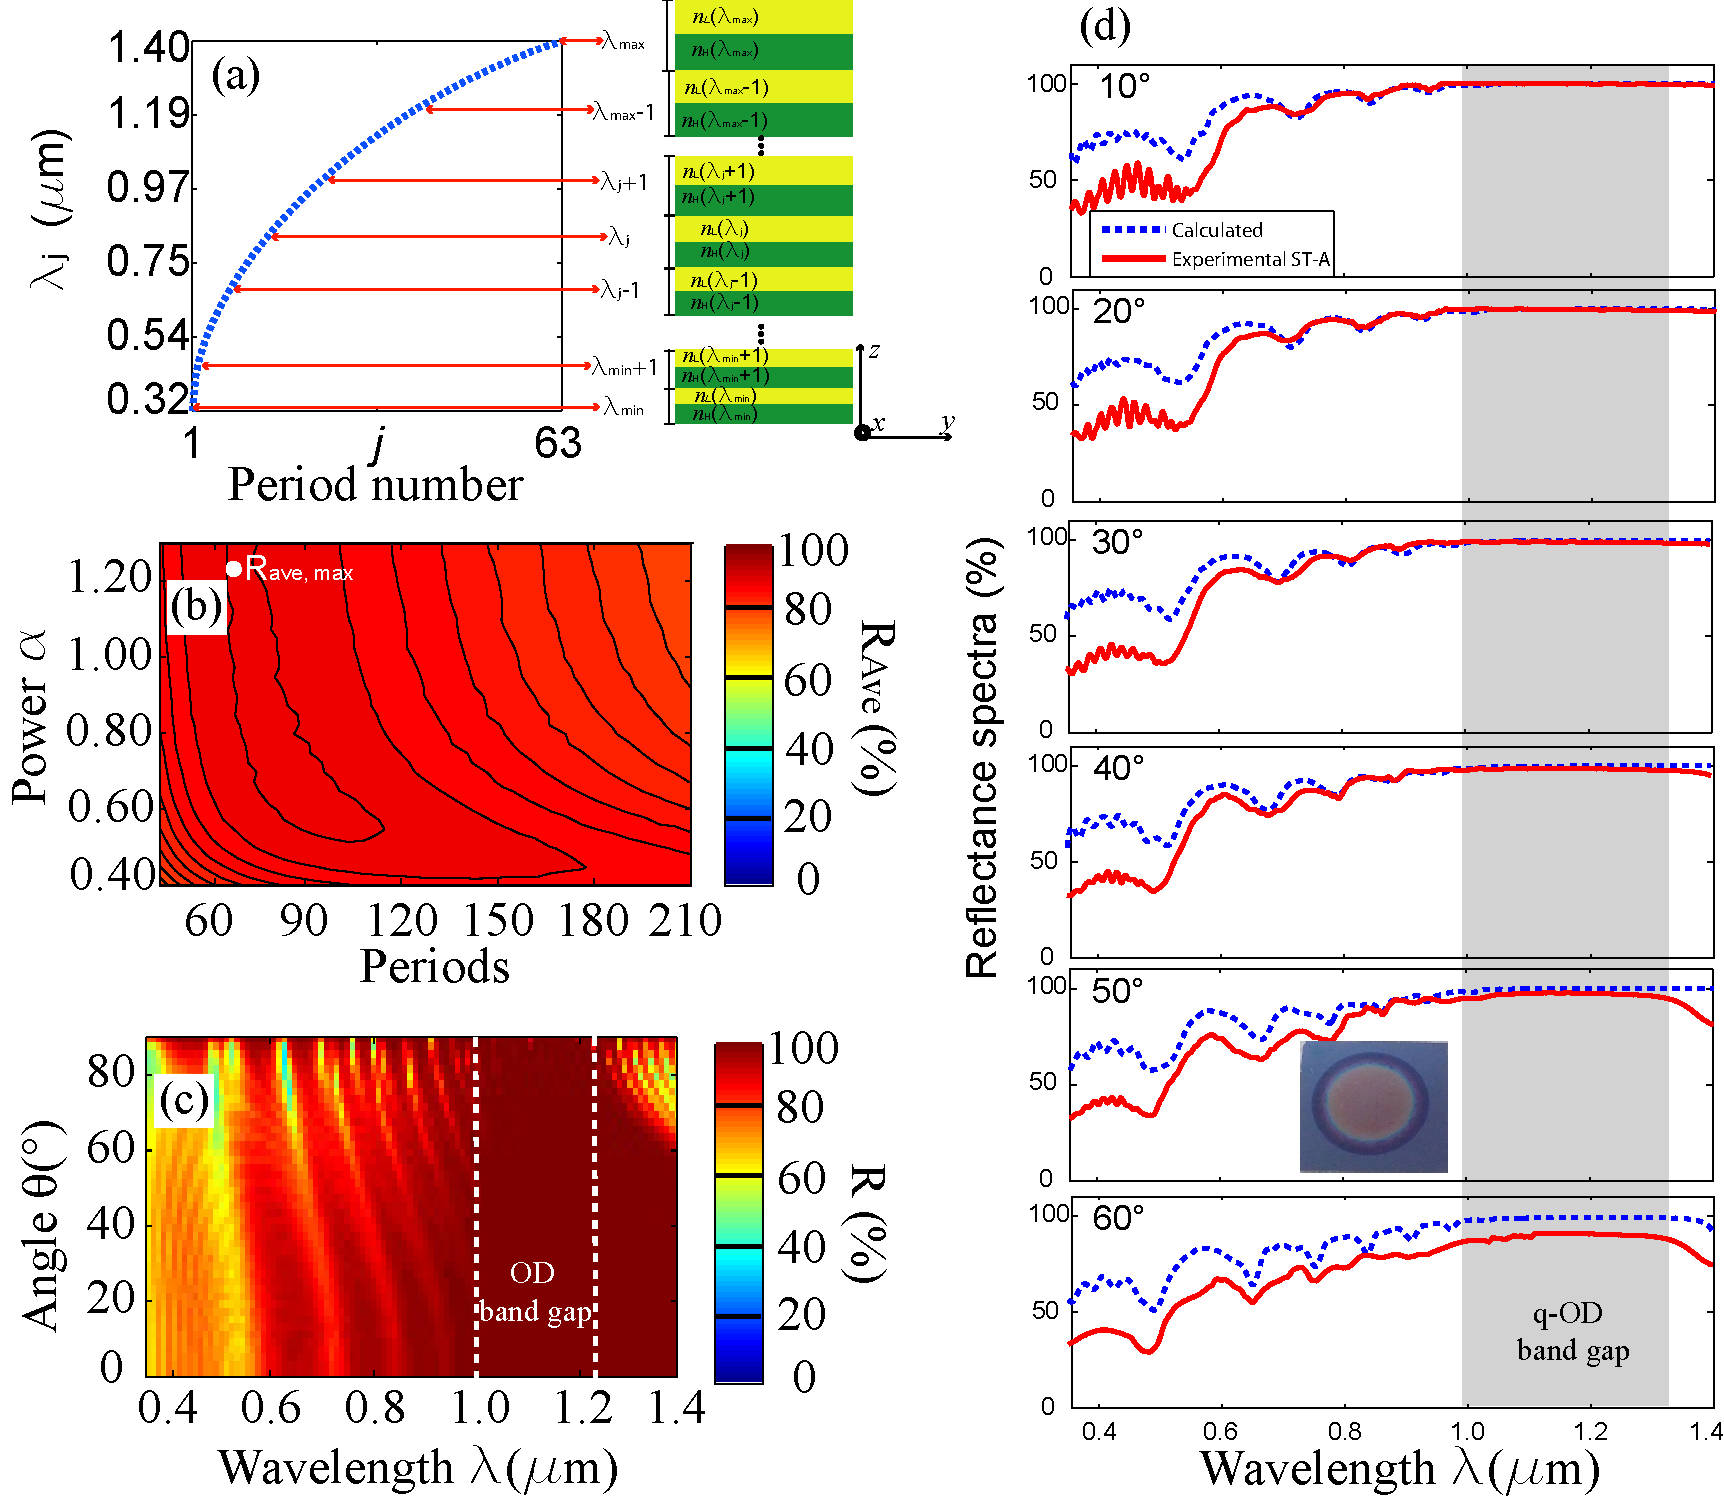
\includegraphics[width=\textwidth]{F3OptimizedVis.pdf}
\end{center}
\caption{(a)Design wavelength $\lambda_{j}$ vs. period number $j$-th
  for the optimized structure ST-A with 63-periods.\notaL{Parece un
    poster miniatura. ¿La ilustración a la derecha está a escala o
    es esquemática? ¿La necesitamos? Está tan chica que es
    ilegible}\notaL{¿Qué es eso de $\lambda+1$? Creo que está mal}
  (b) Average reflectance of the structures designed with different
  values of $\alpha$ and $N_{p}$.\notaL{Por qué en la misma figura?
    ¿Cuál es el propósito de incluir esta? Cambia el cbrange para que
    el color diga algo. Se ve todo rojo uniforme.} It is verified that the
  parameters obtained during the optimization are adequate ($\alpha
  =1.23$ and $N_{p}=63$).\notaL{Este comentario va en el texto, no en
    el pie de figura} (c) Reflectance for non polarized light of the
  optimized structure. (d) Comparison of the reflectance spectra
  calculated and measured at different angles of incidence. The gray band indicates the
  region in which the reflectance is greater than 95\%. Inset shows the
  top view photograph of the synthesized structure.\notaL{En mi
    humilde opinión son demasiadas figuras en una sola, no
    claramente relacionadas entre sí.}}
\label{Fig2}
\end{figure}
In Fig. \ref{Fig2}(b)
we show $\braket{R}$ for different values of $N_p$ and
$\alpha$ to illustrate its dependence on the parameters, and
to verify that our optimized values correspond indeed to the maximum. Here, the
parameters $\lambda_{\text{min}}$, $\lambda_{\text{max}}$, $\beta$ and $A$ were
adjusted, while $N_{p}$ and $\alpha$ varied from 30 to 200 periods and from 0.4 to 1.3,
respectively. \notaL{Ya no me quedó claro. Hay que decir arriba cuales
  son los parámetros que se variaron durante la optimización original. ¿Fueron
  $N_p$, $\lambda_{min}$, $\lambda_{\max}$, $A$, $\alpha$ y $beta$,
  todos ellos? Creo que no es claro. Si fue así, hay que distinguir
  las longitudes de onda del ajuste de las del rango en que
  optimizaste la reflectancia}
The calculated reflectance, $R(\lambda ,\theta)$ of the optimized
photonic structure is shown in Fig \ref{Fig2}(c) for wavelengths and incidence
angles covering the ranges from 350 to 1400 nm, and from $0^\circ$ to $90^\circ$,
respectively. Calculations indicate that the structure is an omnidirectional
mirror with a  reflectance $R>0.95$ within a band from 1000 to 1200
nm. \notaL{La zona gris en la figura va más allá de 1200.} We
fabricated a sample corresponding to our
optimized structure and measured its reflectance spectra at several
incidence angles $\theta$. Due to
experimental limitations, we restrict our results to the case of
non-polarized light.
In Fig. \ref{Fig2}(d), the calculated and
measured reflectance are compared
for $\theta=10^\circ$, $20^\circ$, $30^\circ$, $40^\circ$, $50^\circ$
and $60^\circ$. In this angular range, the structure has a
quasi-omnidirectional band gap (R$\left(\lambda,\theta\right)>95\%$) located from
980 to 1340 nm. \notaL{Aquí hay un error: el experimento salió ¡mejor
  que la teoría! (ver arriba) Algo hay mal en la descripción, pues la
  figura muestra al experlimento abajo de la teoría.}  The
numerical and experimental spectral line shapes at different
angles are in good agreement. For $\lambda>700$nm and
$10^\circ<\theta<40^\circ$ the spectra differs by
less than $5\%$. For $\theta>40^\circ$ both spectra agree
qualitatively but the measured reflectance is lower that than the
calculated one. This difference can be attributed, in part,
to the scattering of light at the actual interfaces, which generally
have some roughness \cite{Theiss1994,Chavez2020} which we have not
accounted for in our theory.\notaL{Quizás aquí puedas citar el
  artículo de Guillermo Ortiz y mío reciente {\em Rough 1D  Photonic
    Crystals: a transfer matrix approach}, Leandro Missoni, Guillermo
  Ortiz, María Martinez Ricci, Victor Toranzos y W. Luis Mochan,
  Optical Materials {\bf 109}, 110012 (2020)
{\tt https://doi.org/10.1016/j.optmat.2020.110012}}

Due to the disipative nature of Si in the UV and the visible region, it is relatively
difficult to design porous silicon omnidirectional mirrors in that region.
However, in the IR region, it is relatively easy to obtain highly reflective
and even omnidirectional photonic structures over a wide
range. \notaL{Está rara la lógica: ¿optimizamos en esa región porque
  es fácil o usamos $f_1$ porque optimizar es fácil? Quizás primero
  debamos decir que nos interesa esa región y que como es fácil,
  usamos $f_1$.}
Therefore,
the reflectance average in the region of 850 to 3000 nm and for all
angles was optimized using the function $f_{1}$ (Eq. (\ref{F1})), yielding
$\alpha=1.2$ with $N_p=90$ and a thickness of 60.4 $\mu$m. \notaL{Aquí
  me vuelve a confundir. ¿90 es el ancho óptimo o
  es el ancho mínimo que permitió... qué?} The resulting design
wavelengths of the structured, designated as ST-B, \notaL{¿Por qué se llaman así? ¿Qué significa
  ST?} are shown in Fig.
\ref{Fig3}(a).
\begin{figure}[tbph]
\begin{center}
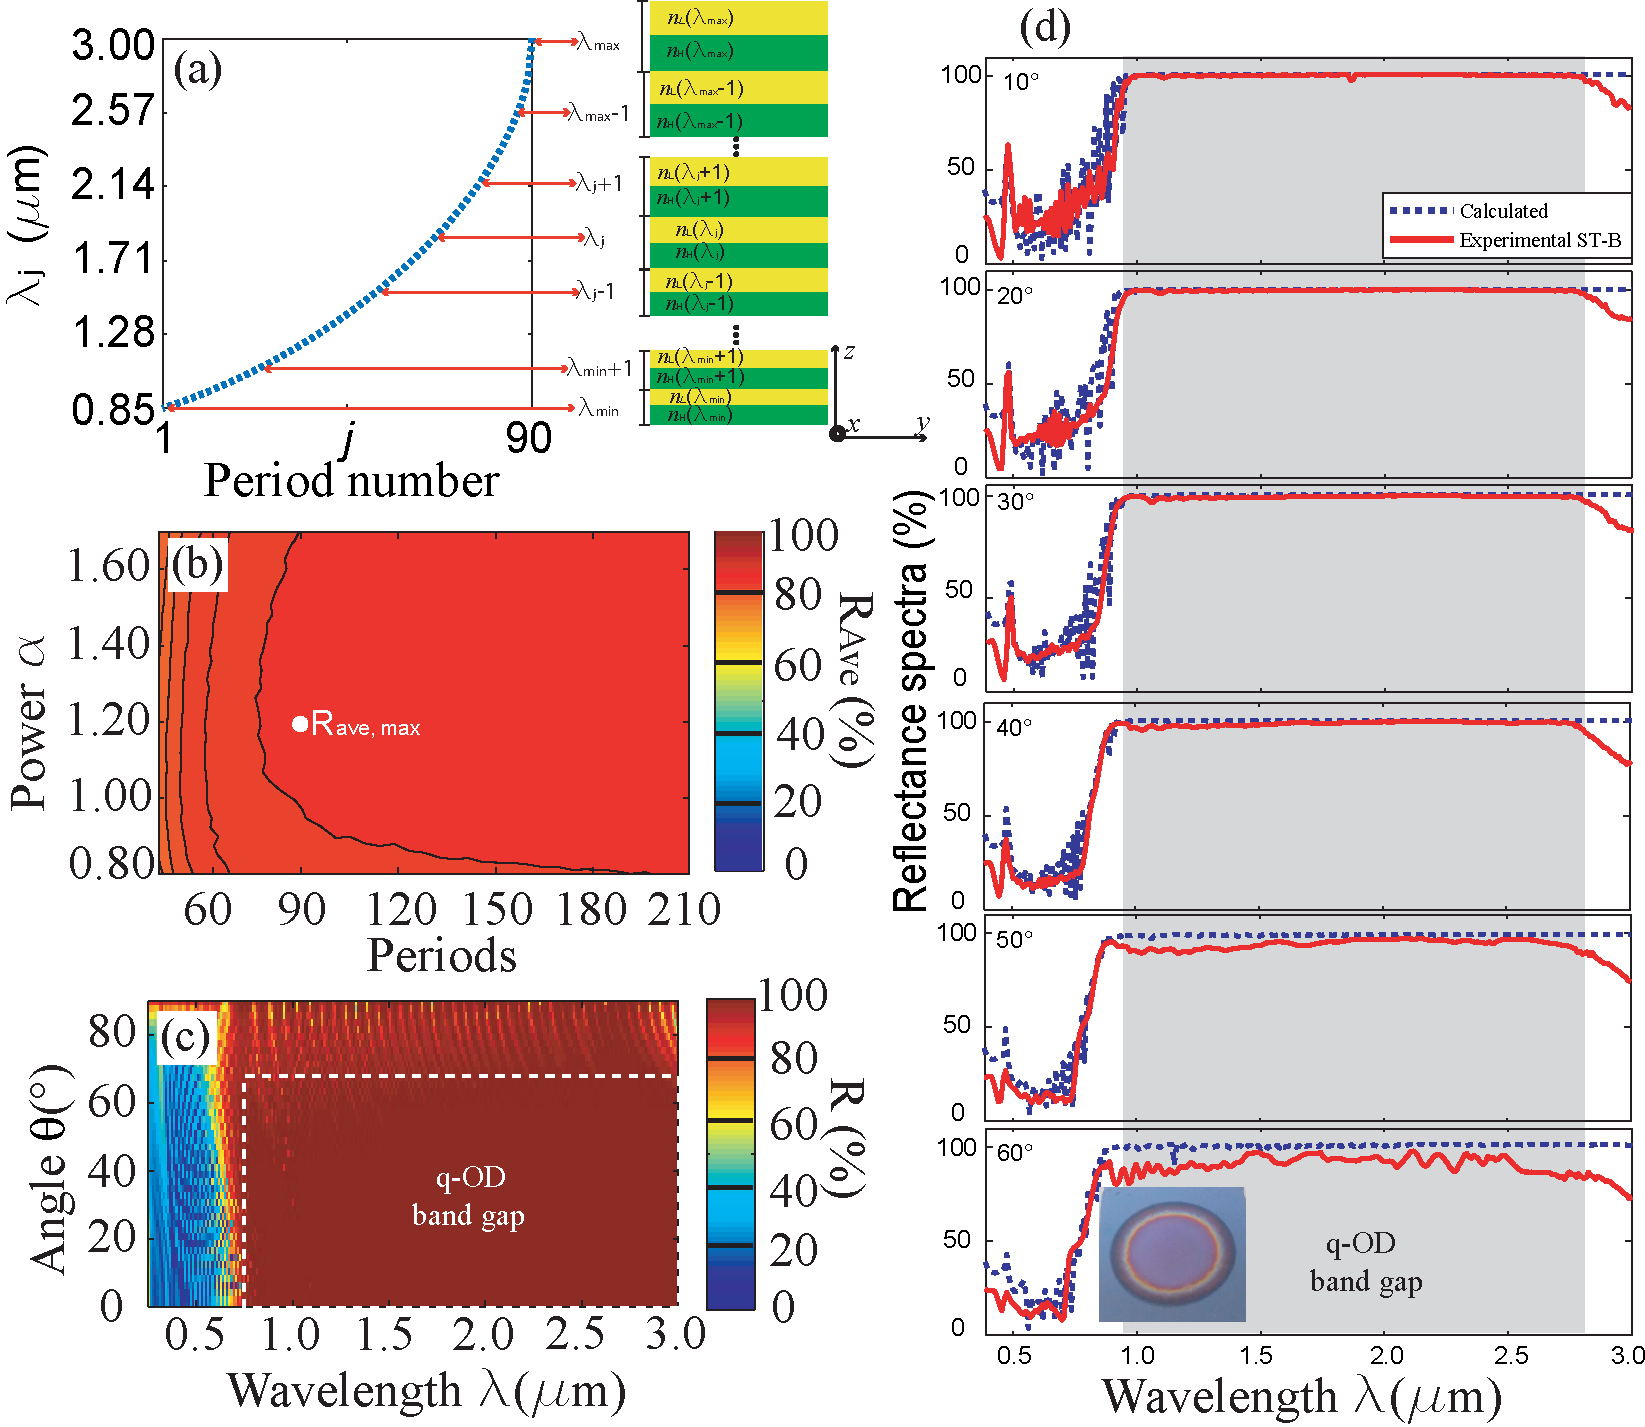
\includegraphics[width=\textwidth]
{F4OptimizedNIRPC.pdf}
\end{center}
\caption{(a) Design wavelengths $\lambda_j$ as a function of period
  number $j$ for sample ST-B. (b) Average reflectance $\braket{R}$
for different values of the parameters $\alpha$
and $N_p$ parameters. \notaL{Cambia el letrero en la figura} The
optimized parameters $\protect\alpha =1.2$
and $N_p=90$ are displayed as a white spot.\notaL{No se ve que sea el
  óptimo. Quizás se necesiten línes de contorno más juntas.} (c)
Calculated reflectance of the optimized
structure for non polarized light.\notaL{¿QUé indica la raya punteada
  y el letrero en la figura?} (d) Comparison of
the calculated and measured spectra  for several angles of incidence. The
gray band indicates the region in which the reflectance is greater than 95$\%$. Inset:
photograph of the synthesized structure.}
\label{Fig3}
\end{figure}

\notaL{Tengo los mismos comentarios que para la figura previa.}
Fig \ref{Fig3}(b) shows $\braket{R}$ for
different values of $\alpha$ and $N_{p}$. As in the
previous case, the optimized parameters are within the zone of maximum
average reflectance. \notaL{No debería ser el mismísimo máximo y no
  nada más en la zona?} The reflectance calculation  is
shown in Fig. \ref{Fig3}(c).  This structure
has a wide quasi-omnidirectional gap with $R(\lambda,\theta)>0.95$
with $\lambda$ from 850 to 3000 nm and $\theta$ from
$0^\circ$ to $70^\circ$.\notaL{Me da la impresión que confundías
  promedio con reflectancia} The measured and calculated reflectance
are compared  for several angles in Fig \ref{Fig3}(d). The synthesized PS
multilayered 1D photonic structure behaves as a quasi omnidirectional
mirror for $0^\circ\le\theta\le 60^\circ$ with a bandwidth of approximately 1800 nm. The difference
between the calculated and measured spectra at the longer wavelengths can be
attributed to a thickness gradient along the depth,\notaL{No entiendo:
  está diseñada para tener un gradiente de ancho. Te refieres a un
  gradiente adicional al diseñado?} which is more pronounced in
the lower layers due to the restricted diffusivity of the electrolyte
through the structure itself \cite{Negro2003,Vincent1993} and
interface roughness \notaL{No se entiende si este es otro efecto o si
  la rugosidad produce un gradiente de anchos}.

\subsection{Photonic structure with sub-mirrors stacking}

Another technique to design Bragg mirrors in a wide range of the
electromagnetic spectrum is by stacking sub-mirrors at different
wavelengths \cite{DelRio2018,Agarwal2003}. Such grouping must meet the condition
imposed by the dispersion relation, $\cos KD=\frac{1}{2}\text{Tr}\,M$, where $D$ is
the period, which corresponds to the actual thickness of the sub-mirror, $\pm K$
represents a 1D Bloch's vector corresponding to a wave that propagates along
$z$-direction \cite{Mochan1987,Mochan1988,Perez2018}, and T$\text{r}$ denotes the
trace. This equation is bounded by the minimum and maximum values that the cosine
function can take. Furthermore, if  the value of $\left\vert \text{Tr}\left(
M\right) \right\vert$ is $>2$, it indicates that this frequency will not
be able to propagate through the structure.

The ideal stack of sub-mirrors would be that PBG of the $j$-th mirror begins
at the edge of the PBG of the $j-1$-th mirror, until the desired interval has been
covered. However, this arrangement does not give the maximum average reflectance due to
the decrease in the reflectance at each intersection of the two PBGs. On the other hand,
the number of periods of each sub-mirror is an important parameter due to its direct
dependence on the magnitude and  width of  the photonic band gap.  As the structures
were synthesized using porous silicon, it is essential to minimize the number of
periods corresponding to the visible region sub-mirrors. Also, in the supplementary
information we show the reflectance calculations for structures composed of sub
mirrors with a constant number of periods, in these cases ODBMs are not obtained.
For these reasons, the number of periods for each mirror was chosen as follows: for
design wavelengths less than 500 nm ($\lambda_{D}<$500 nm), one period, for 500
$<\lambda_{D}<$650 nm, two periods , for 650 $<\lambda_{D}<$800 nm, three, and for
$\lambda_{D}>$ 800 nm, the number of periods was variable (Fig. \ref{Fig4}(a)).
\begin{figure}[tbph]
\begin{center}
\includegraphics[width=\textwidth]
{F6OptimizedNIRSE.pdf}
\end{center}
\caption{(a) Diagram showing the distribution of sub-mirrors and the corresponding
number of periods in a PS multilayer. (b) Maximization of the average reflectance as
a function of the overlap photonic band gap for the structures formed by sub-mirrors
with a fixed number of periods (3 and 4), and for structures with the design of (a)
using 3 and 6 periods for the tuned sub-mirrors in $\lambda>800$ nm. (c) Mapping the
calculated reflectance of the designed structure with the optimized values for non
polarized light. (d) Comparison of reflectance spectra calculated and measured at
different angles of incidence. The gray band indicates the region in which the
reflectance is greater than 95$\%$. Inset shows the top view photograph of the
synthesized structure.}
\label{Fig4}
\end{figure}

Therefore, in this work the overlap percentage of the PBGs of the first and second
mirror, second and third mirror, and so on, is also optimized. Fig \ref{Fig4}(b)
shows the optimization results in terms of maximum average reflectance with respect
to the PBG overlap at different sub-mirror periods, keeping them fixed (3, 4) or
variable (1, 2  and 3) for $\lambda<500$(1 period), $500<\lambda<650$ nm (2
periods), $650<\lambda<800$ nm (3 periods) and $\lambda>800$ (3, 6 periods). For
example, the calculations corresponding to the reflectance spectra of the structures
formed using sub-mirrors with constant periods (3 and 4) revealed a lower average
reflectance as compared to the structure formed with variable periods. The 1D
photonic structure with the highest average reflectance (named as ST-C)  is the one
designed with variable periods and contemplates 6 periods for each sub-mirror in the
NIR region. In the optimized structure designed for 400-3000 nm range, the photonic
band gap overlap is around 78$\%$, thickness is 41.5 $\mu $m and the average
reflectance is 95.3$\%$, when the  electromagnetic waves are incident from
0${{}^\circ}$ to 89 ${{}^\circ}$. The optimized photonic structure is made up of 18
sub-mirrors tuned to the following wavelengths 400, 460, 510, 570, 640, 720,810,
910, 1020, 1150, 1290, 1450, 1630, 1830, 2060, 2320, 2610 and 2860 nm  with periods
of 1 (400, 460 nm), 2(510, 570, 640 nm), 3 (720 nm) and 6 (810 nm and above).

The reflectance mapping shown in Fig \ref{Fig4}(c) reveals a quasi omnidirectional
band gap from 950 to 2900 nm, taking into account 0${{}^\circ}$ to 60${{}^\circ}$ of
incidence. It is also observed that at incidence angles $>$70${{}^\circ}$, for long
wavelengths the reflectance decreases and has oscillations, which are attributed to
the greater penetration of the electromagnetic field within the structure, as shown
by Puente-D\'{\i}az, et al \cite{Puente2020}. Furthermore, in supplementary
information we show the transfer matrix trace calculations as a function of the
wavelength and the incidence angle for the ST-C photonic structure using the TE and
TM polarization. In Fig \ref{Fig4}(d) the calculated and measured reflectance
corresponding to the structure ST-C, at different angles of incidence is compared.
Although, the quasi omnidirectional band gap of the synthesized structure is
slightly less than that calculated (located from 950 to 2750 nm), the measured PBG
is almost twice as compared to the recently reported similar structures
(\cite{DelRio2018,Chavez2020}).

Finally, table 2 shows some porous silicon based ODBMs designed to operate in the
NIR region and the width of the omnidirectional band gap is compared with the
structures analyzed in the present study. The table reveals that the porous silicon
based structures ST-B and ST-C have the widest gap width, being 1.8 times greater
than recently reported works.

\begin{table}[h!]
	\begin{center}
		\caption{Summary of the development in porous silicon based ODBMs designed in the NIR region.}
		\label{tab:table1}
		\begin{tabular}{c|c|c|c}
			\hline % <-- Toprule here
		\textbf{Reference}&\textbf{Year}&\textbf{ODBM range}&\textbf{ODBM width}\\
			 & &(nm)&(nm)\\%&\textbf{ST-B}&\textbf{ST-C}\\
			\hline % <-- Midrule here
Bruyant, et al \cite{Bruyant2003}. & 2003 & 1100-1440 & 340 \\
Xifre-P\'{e}rez, et al \cite{Xifre2005}. & 2004 & 1297-1615 & 318\\
Estevez, et al \cite{Estevez2009}. & 2009 & 950-1456 & 506 \\
Chavez, et al \cite{Chavez2020}. & 2020 & 1000-2000 & 1000 \\
			\hline % <-- Bottomrule here
			\begin{tabular}{c|c}
					&ST-A\\
					This article&ST-B\\
				&ST-C\\
			\end{tabular}&
			\begin{tabular}{c}
			\\
			\\
			\\
			\end{tabular}&
		\begin{tabular}{c}
			980-1340\\
			980-2780\\
			950-2750\\
		\end{tabular}&
		\begin{tabular}{c}
			360\\
			1800\\
			1800\\
		\end{tabular}\\
		\hline % <-- Bottomrule here
	\end{tabular}
	\end{center}
\end{table}


\section{Conclusion}\label{s:conc}

We have demonstrated the formation of highly reflective PS multilayer photonic
structures optimized using two types of design techniques for maximal reflectance
and minimal thickness in the NIR region. With \textit{chirped}-type Bragg mirrors,
two regions of the electromagnetic spectrum were analyzed. The first region (350nm -
1400 nm), optimized through an increasing function resulted in an average
reflectance $>85\%$ with the quasi omnidirectional PBG of 360 nm centered at 1160 nm
(980-1340 nm) for the angular range 0-60${{}^\circ}$ and more than 50$\%$ of
reflectance from 550-980nm. The second structure was designed for 850-3000 nm
wavelength range and the synthesized structure with optimized parameters resulted in
the average reflectance of $~91\%$ with q-OD bandgap from 980 to 2780 nm and a
thickness of 60.4 $\mu$m. The other design technique consisting of sub-mirrors
stacks (designed at different wavelengths), was optimized for maximum average
reflectance with respect to the percentage overlap of the PBG for each sub-mirror. A
multilayer structure using the optimized parameters with sub-mirrors stack method
was obtained with the average reflectance of $~95\%$ and a thickness of 41.5 $\mu$m.
Furthermore, this structure revealed a 1800 nm q-OD PBG, centered at 1850 nm, in
angular range 0-60${{}^\circ}$. Therefore, this second technique was found to be
better due to the decreased thickness (by a factor of $~1.5$) of the framework and
increased average reflectance. Additionally, the analysis techniques developed here
can be used to optimize reflectance with other refractive index contrasts in PS
multilayers or different other systems composed of other types of materials. Such
proposed structures could be used as mirrors for solar concentrators, flat focusing
reflectors, thermal regulators, or, if defects are included, as filters or remote
chemical/biosensors with a wide angular independent response.



\section*{Acknowledgments}
This work was partially supported by Consejo Nacional de Ciencia y
Tecnolog\'{i}a through grant No. \textbf{256243} and C\'{a}tedras
Conacyt program 1577, and by DGAPA-PAPIIT UNAM under grant IN111119.
%\end{acknowledgments}

\bibliographystyle{unsrt}
\bibliography{Bibliografia}
\end{document}
